\documentclass[twoside]{article}
\usepackage{seminarpaper, dirtytalk, graphicx,algorithm,amsmath,amsfonts, tabularx, subcaption}
\usepackage[noend]{algpseudocode}

\usepackage[style=authoryear-icomp, maxbibnames=9, maxcitenames=2, backend=biber]{biblatex}
\addbibresource{seminarpaper.bib}

\begin{document}

% If your paper is accepted and the title of your paper is very long,
% the style will print as headings an error message. Use the following
% command to supply a shorter title of your paper so that it can be
% used as headings.
%
%\runningtitle{I use this title instead because the last one was very long}

% If your paper is accepted and the number of authors is large, the
% style will print as headings an error message. Use the following
% command to supply a shorter version of the authors names so that
% they can be used as headings (for example, use only the surnames)
%
%\runningauthor{Surname 1, Surname 2, Surname 3, ...., Surname n}

\twocolumn[

\papertitle{Computational Challenges in Navigation}

\paperauthor{ Andrew J. Kronser }
\paperaddress{ } ]

\begin{abstract}
\large
  There are many challenges in obtaining navigation solutions from smartphone sensors.
  This was the topic of the intensive Computational Challenges in Navigation course.
  This summary will summarize the content of the course and then survey the topic of
  pedestrian navigation.
\end{abstract}

\section{INTRODUCTION}
\large
Modern smartphones are constantly being used for navigation. They come equipped with
a wide array of sensors that allow for satellite, network, and inertial information
to be processed into a navigation solution. These sensors are often small and low-cost
in order to meet size and cost requirements and therefore have limited accuracy. It's
highly important to use multiple sensors to obtain more accurate navigation solutions.

Since Google opened an API for raw Global Navigation Satellite System (GNSS) measurements,
researchers have been able to use Android devices (at least those that support the API)
to collect GNSS measurements for further processing with measurements from other smartphone
sensors including inertial (INS) sensors. These measurements can be combined with other
sensory data using Kalman filtering.

With access to more raw GNSS data, it's possible to better research how smartphone-based
navigation solutions can be improved.
\subsection{GNSS}
GNSS refers to radio receivers that process signals from navigational satellite constellations
(GPS, GLONASS, Gallileo, BeiDou). At least four signals are needed to give a position solution.
Four signals form a specified system for the four unknowns (x, y, z, and receiver clock bias).

The signal consists of three layers. The carrier signal is the base frequency of the signal
common to all satellites in the constellation except in the case of GLONASS which uses the base
signal to distinguish between satellites, a system known in general as frequency
division multiplexing (FDM). In other systems, the pseudorandomly generated C/A layer is used
instead to identify each satellite uniquely.

In either case, on top of these two layers is the navigation layer which contains position information
(ephemeris) for the satellite, clock corrections, and information about the other satellites in the
constellation (almanac). The ephemeris data can also be obtained over the Internet (this is useful
in mobile applications because otherwise it would take a minimum of 18 seconds to determine
the GNSS solution).
\subsection{INS}
Inertial sensors give information about the relative position of a body in space. For smartphone
applications, we're concerned with the smartphone's accellerometer (which measures change in position)
and gyroscope (which measures change in attitude). Taken together, these sensors can give a user's
relative position over time without any external reference.

The problem with relying on INS sensory data is that the navigation solution deteriorates quickly
without external reference since the solution is based on a dependent series of measurements (unlike
GNSS where individual measurements are independent), so errors propagate as time progresses.
Within a matter of seconds, the necessary accuracy for most navigation tasks is lost.

In order to make use of inertial measurements, GNSS and other absolute position data can be used
to correct errors. Then, INS data can be used when GNSS services are unavailable.
\subsection{WLAN, Bluetooth, and LAN}
Network based solutions, though not the focus of the course or this summary, are also frequently used
to augment indoor navigation solutions. The primary problem with these solutions is availability
and reliability.
\subsection{Computer Vision}
Another form of sensory data that can be used to augment navigation solutions is computer vision.
The use of computer vision techniques to augment navigational data is commonly seen in applications
for autonomous vehicles.
\subsection{Navigationally Challenging Environments}
In outdoor settings with clear visibility of the sky, GNSS navigation is reliable. Urban environments,
on the other hand, are more challenging. GNSS signals aren't reliable in urban canyons where multipath
interference from signals bouncing off buildings is common. GNSS also isn't available in indoor settings.

In these more challenging environments, other means of navigation (computer vision, inertial sensors, and
other radio networks) must be used to augment the solution when GNSS isn't available or reliable.

Another challenging environment is potential interference through jamming or spoofing. Since modern
industrial and military equipment is dependent on GNSS-based navigation, these systems are a target
for attacks. Jamming targets GNSS availability by flooding the relevant bandwidth with noise. Spoofing,
unlike jamming, imitates the GNSS signal to mislead the receiver into believing that it's in a different
position. This makes spoofing attacks particularly dangerous.
\section{COMPUTING NAVIGATION SOLUTIONS}
\subsection{GNSS}
Android's raw GNSS measurements API provides pseudorange estimates, pseudorange rates, and hardware clock
information. Depending on the device's hardware, some or all of this information may be available.

The pseudoranges provides include error (from ionospheric interference, tropospheric interference, and
miscellaneous errors) and therefore must be corrected. After correcting a position solution is can be
determined by optimizing the following system of equations.

\begin{align*}
    \hat{x} = \langle \delta \mathbf{x}, \delta b\rangle = (\mathbf{G}^T\mathbf{G})^{-1}\delta\mathbf{\rho} 
\end{align*}

Where $\mathbf{x}$ is the true position, $\hat{x}$ is the position estimate, $\mathbf{G}$ is the geometry matrix,
and $\rho$ is the pseudorange vector. A weighted least squares solution is used instead to account
for measurements of differing quality from different satellites. This solution also must be corrected for the
rotation of the earth that occurred during propagation.

Velocity estimates can be obtained by solving a similar system.

We can express the signal quality of GNSS measurements using carrier-to-noise-density ratios $C/N_0$. These
ratios can indicate which signals should be used and whether enough strong signals are present to compute
a meaningful navigation solution.
\subsection{INS}
Inertial computation uses measurements from the inertial measurement unit (IMU) inside of the smartphone.
These measurements need to first undergo a series of frame transformations in order to go from the body
frame (in which they are measured) to the navigation frame (latitude, longitude, altitude). The accelerometer
doesn't measure position, however, it measures acceleration and therefore needs to be adjusted for local
gravity, the rotation of the earth, and the Coriolis effect. Attitude (which is needed for these transformations)
requires initialization to an absolute reference (by magnometer for example) and is tracked by the gyroscope.
Position and velocity also need to be initialized. Initial postion can be supplied by GNSS and initial velocity
can be set by having the user stand still.
\subsection{Kalman Filtering}
Kalman Filtering is used to combine measurements from different sensors in a process. It's a simple algorithm
that alternates a priori (prediction) and a posteriori (measurement correction) updates. More formally, we
estimate a state $\mathbf{x}_k \in \mathcal{R}^n$ using a state transition matrix $A$, weighted control input
$B\mathbf{u}_{k - 1}$, and process noise $w_{k - 1} \sim \mathcal{N}(0,Q)$. Measurement is modelled using an
observation model $H$ and measurement process noise $\mathbf{v}_k \sim \mathcal{N}(0,R)$
\begin{align*}
    \mathbf{x}_k &= A\mathbf{x}_{k-1} + B\mathbf{u}_{k - 1} + \mathbf{w}_{k - 1} \\
    \mathbf{z}_k &= H\mathbf{x}_{k-1} + \mathbf{v}_k
\end{align*}

For each time step, $k$, this yields the following updates for the \say{predict} step,
\begin{align*}
    \hat{x}_k^- &=  A\hat{x}_{k - 1} + Bu_{k - 1} \\
    P_k^- &= AP_{k - 1}A^T + Q
\end{align*}

and the following updates (optimisations) for the \say{correct} step.
\begin{align*}
    K &= P_k^-H^T(HP_k^-H^T + R)^{-1}\\
    \hat{x}_k &= \hat{x}_k^- + K_k(z_k - H \hat{x}_k^-)\\
    P_k &= (I - K_kH)P_k^{-}
\end{align*}

The state transition matrix needs to be initialized to model the process (in our case, INS and GNSS
measurements for navigation). It's also extremely important to pick a good initialization for the process
noise covariance $Q$ though the criteria used were beyond the scope of our course.

Kalman filters can take as input raw or processed GNSS data. The level of coupling of a Kalman filter
describes the amount of data preprocessing prior to input to the Kalman filter. In the case of GNSS,
deeply-coupled Kalman filters take raw GNSS signals whereas loosely couple Kalman filters use position
solutions as input. For our experiments, we used tightly coupled Kalman filtering, where the carrier
phase and range measurements were used as inputs to fuse with GNSS data.
\section{EXPERIMENTS}
In order to better understand the collection of GNSS and INS measurements and their fusion we conducted
experiments during the course. My application (pedestrian navigation) lead me to collect data on different
forms of modal public transport (walking, tram, and bus) to see the availability of GNSS in each of these
situations. Data was collected along a short, straight-shot route in Arabia. Two sets of inertial and
GNSS data were collected for each mode of transportation. The resulting data was fused using tightly-coupled
Kalman filtering.

Since the time frame for planning and executing these tests was relatively short, the results weren't very
conclusive. The fusion solution paths deviated heavily due to a lack of GNSS availability in either vehicular
mode. On the other hand, this was the most illustrative part of the results. Even with minimal obstruction
(such as a vehicle) GNSS signal strength is unreliable. This can be demonstrated from the
carrier-to-noise-density ratios of walking compared to riding the tram.

\begin{figure}[H]
\centering
\begin{subfigure}[b]{0.5\textwidth}
   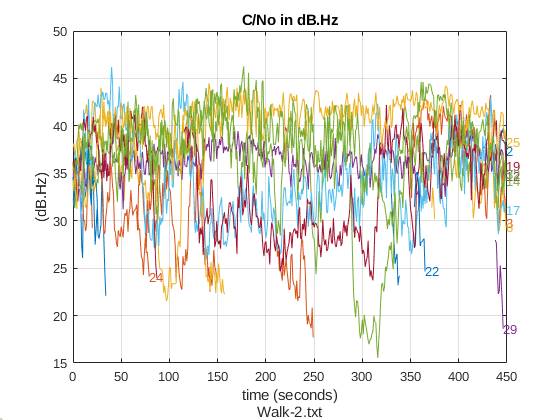
\includegraphics[width=1\linewidth]{CNo-Walk-2.png}
   \caption{}
   \label{fig:Ng1} 
\end{subfigure}

\begin{subfigure}[b]{0.5\textwidth}
   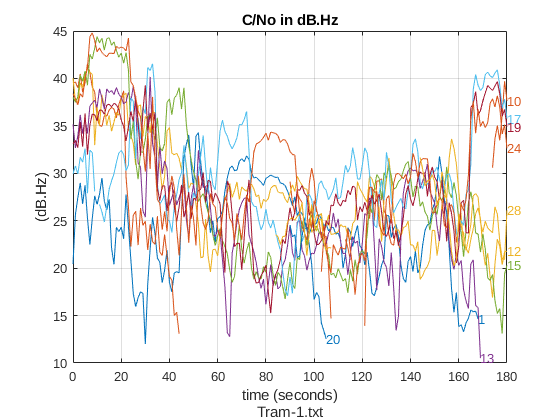
\includegraphics[width=1\linewidth]{CNo-Tram-1.png}
   \caption{}
   \label{fig:Ng2}
\end{subfigure}

\caption[Two numerical solutions]{(a) Carrier-to-noise-density ratios for GNSS signals for the walk
path (b) for the tram path}
\end{figure}

Because of these challenges, additional steps need to be taken in order to make urban pedestrian navigation
with smartphones more reliable and more accurate.
\section{PEDESTRIAN APPLICATION}
In the papers provided and the supplemental material during Friday's lecture, several methods were presented
that could increase the accuracy of smartphone navigation to a level more applicable for pedestrian application
in navigationally challenging environments. Two of these technologies, assisted GNSS, and
5G, require infrastructure to assist the current GNSS and smartphone sensory array. The other technology,
precise point positioning (PPP), doesn't require additional infrastructure but only displayed more encouraging
results (with smartphone sensors) in static settings.
\subsection{Assisted GNSS}
In an assisted GNSS setting, ephemeris and almanac data is supplied by an external server (such as over-the-air
information provided by a mobile carrier). This can improve several metrics, especially the time to first
fix (a fraction of a second as opposed to 18 seconds to obtain ephemeris data). The position server also
computes the position solution easing the computational needs of the mobile station.

Though this can improve time to first fix which is very useful for pedestrian applications, the improvement
in accuracy is insufficient for navigation and assisted GNSS depends on position server infrastructure
availability and reliability.
\subsection{5G}
Though 5G networks are in development in many places, 5G has promising applications for pedestrian
navigation. 5G access nodes (ANs) deployed in ultra-dense small cells could provide sub-meter accuracy for
mobile positioning (\cite{5G}). 

Tracking an user network (UN) can be done using Kalman filtering to perform location tracking, efficiently
predicting where the UN will move in relation to the AN. This makes sense because a user's motion is a
discrete-time process (just as it was for GNSS/INS fusion).

There are several drawbacks, however, to 5G solutions. In particular, indoor penetration
isn't very good because positioning requires line-of-sight signals. Another major problem with 5G
positioning is that no real-world testing has been as of now. Testing in controlled environments and
simulations is unlikely to well-replicate real-world conditions. This makes 5G promising going forward,
but the technology is far from being widely-available.

Should ultra-dense 5G networks become commonplace, their application to pedestrian navigation is somewhat
obvious. In urban settings (where ultra-dense 5G is most likely to be deployed), 5G positioning can mitigate
the impacts of navigationally challenging environments such as urban canyons. The short-range signal also
makes 5G navigation less susceptible to widespread spoofing or jamming.
\subsection{PPP}
Precise point positioning (PPP) also has promising applications for smartphones going forward. Though
most smartphones are bound by a duty cycle (where GNSS sensors are only activated infrequently to
save power), at least one phone, the Xiaomi Mi 6, allows this duty cycle to be disabled, which makes
PPP more viable (\cite{PPP}).

PPP uses carrier-phase information in addition to pseudorange information in order to generate a GNSS
position solution. Carrier-phase information is the range between a user and satellites as expressed
in units of carrier frequency cycles. Resolving the ambiguity between cycles can be difficult because
of measurement error.

It has been demonstrated, however, that smartphones in a static setting can have their position estimated
to a high accuracy. Though this result alone doesn't bear much for pedestrian applications (which are
usually dynamic in nature) further developments are more phones allow duty cycling to be disabled could
lead to non-static applications of PPP. Non-static applications deviate by 4-6 meters in outdoor environments
which is akin to the accuracy for plain GNSS/INS fusion solutions.

PPP also doesn't assist in navigationally challenging environments since it's dependent on GNSS availability.
So while it might help precise positioning in outdoor environments (and may mitigate multipath in denser
urban environments), PPP alone in smartphones doesn't address many challenges with pedestrian navigation.
\section{CONCLUSION/PERSONAL REMARKS}
This course provided a helpful overview to navigational data processing. After taking this course, I have
a deeper understanding of how navigational measurements are taken, processed, and combined with other data
in order to develop robust navigation solutions.

In pedestrian applications, it will be exciting to see how 5G and other emerging technologies change the
landscape of urban navigation. I was unaware of just how inaccurate smartphone GNSS data really was. This
course gave me a greater appreciation for my ability to navigate using only the very cheap equipment in
my pocket. Thanks for an excellent and engaging course.
\subsubsection*{References}
\printbibliography[heading=none]

\end{document}
